\begin{figure}[htbp]
\centering
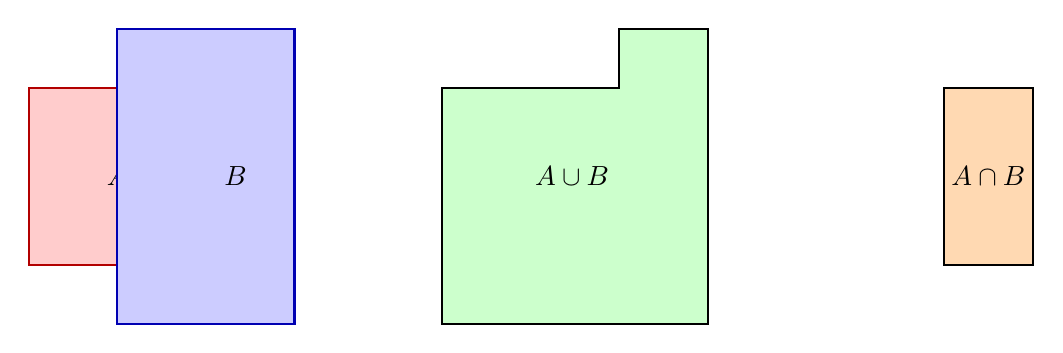
\begin{tikzpicture}[scale=0.75]
  \fill[red!20] (0,0)--(0,3)--(3,3)--(3,0)--cycle;
  \draw[thick,red!70!black] (0,0)--(0,3)--(3,3)--(3,0)--cycle;
  \node at (1.5,1.5) {$A$};
  \fill[blue!20] (1.5,-1)--(1.5,4)--(4.5,4)--(4.5,-1)--cycle;
  \draw[thick,blue!70!black] (1.5,-1)--(1.5,4)--(4.5,4)--(4.5,-1)--cycle;
  \node at (3.5,1.5) {$B$};
  \begin{scope}[xshift=7cm]
    \fill[green!20] (0,-1)--(0,3)--(3,3)--(3,4)--(4.5,4)--(4.5,-1)--cycle;
    \draw[thick] (0,-1)--(0,3)--(3,3)--(3,4)--(4.5,4)--(4.5,-1)--cycle;
    \node at (2.2,1.5) {$A \cup B$};
  \end{scope}
  \begin{scope}[xshift=14cm]
    \fill[orange!30] (1.5,0)--(1.5,3)--(3,3)--(3,0)--cycle;
    \draw[thick] (1.5,0)--(1.5,3)--(3,3)--(3,0)--cycle;
    \node at (2.25,1.5) {$A \cap B$};
  \end{scope}
\end{tikzpicture}
\caption{Polygon boolean operations: Union $A \cup B$ (center) and Intersection $A \cap B$ (right) of two overlapping rectangles.}
\label{fig:polygon_boolean}
\end{figure}
